%%\documentclass[preprint,authoryear,12pt]{elsarticle}
%% Use the option review to obtain double line spacing
\documentclass[authoryear,preprint]{elsarticle}

%% Use the options 1p,twocolumn; 3p; 3p,twocolumn; 5p; or 5p,twocolumn
%% for a journal layout:
%% \documentclass[final,authoryear,1p,times]{elsarticle}
%%\documentclass[final,authoryear,1p,times,twocolumn]{elsarticle}
%% \documentclass[final,authoryear,3p,times]{elsarticle}
%%\documentclass[final,authoryear,3p,times,twocolumn]{elsarticle}
%% \documentclass[final,authoryear,5p,times]{elsarticle}
%%\documentclass[final,authoryear,5p,times,twocolumn]{elsarticle}
\usepackage{tikz}
\tikzset{every picture/.style={line width=0.75pt}} %set default line width to 0.75pt   
%% if you use PostScript figures in your article
%% use the graphics package for simple commands
%%\usepackage{graphics}
%% or use the graphicx package for more complicated commands
\usepackage{graphicx}
\usepackage{subcaption}
%% or use the epsfig package if you prefer to use the old commands
%% \usepackage{epsfig}
\usepackage[fleqn]{amsmath}
%% The amssymb package provides various useful mathematical symbols
\usepackage{amssymb}
%% The amsthm package provides extended theorem environments
\usepackage{amsthm}

\newtheorem{theorem}{Theorem}
\newtheorem{corollary}{Corollary}[theorem]
\newtheorem{lemma}[theorem]{Lemma}
\newtheorem{proposition}{Proposition}

\DeclareMathOperator*{\argmin}{arg\,min}
%% The lineno packages adds line numbers. Start line numbering with
%% \begin{linenumbers}, end it with \end{linenumbers}. Or switch it on
%% for the whole article with \linenumbers after \end{frontmatter}.
%% \usepackage{lineno}

%% natbib.sty is loaded by default. However, natbib options can be
%% provided with \biboptions{...} command. Following options are
%% valid:

%%   round  -  round parentheses are used (default)
%%   square -  square brackets are used   [option]
%%   curly  -  curly braces are used      {option}
%%   angle  -  angle brackets are used    <option>
%%   semicolon  -  multiple citations separated by semi-colon (default)
%%   colon  - same as semicolon, an earlier confusion
%%   comma  -  separated by comma
%%   authoryear - selects author-year citations (default)
%%   numbers-  selects numerical citations
%%   super  -  numerical citations as superscripts
%%   sort   -  sorts multiple citations according to order in ref. list
%%   sort&compress   -  like sort, but also compresses numerical citations
%%   compress - compresses without sorting
%%   longnamesfirst  -  makes first citation full author list
%%

%%\usepackage[table]{xcolor}
\usepackage{tabularx}
\usepackage{enumitem}

\biboptions{square,comma,numbers}

% \biboptions{}

\journal{ }

\begin{document}
	
	\begin{frontmatter}		
		\title{A Model for COVID-19 with Control Measures and Mobility}
		
		\author[a1]{Subhas Kumar Ghosh\corref{cor1}}
		\ead{subhas.ghosh@cba.com.au}
		\author[a2]{Sachchit Ghosh}
		\ead{sgho2841@uni.sydney.edu.au}
	
		
		\cortext[cor1]{Corresponding author}
		\address[a1]{Commonwealth Bank of Australia, Sydney, New South Wales, 2000, Australia}
		\address[a2]{The University of Sydney, Camperdown, NSW 2006, Australia}
	
		
		\begin{abstract}
		\end{abstract}
		
		\begin{keyword}
			COVID-19 \sep SARS-CoV-2 \sep Mathematical modeling \sep Epidemic \sep Intervention \sep Mobility			
		\end{keyword}
		
	\end{frontmatter}
	
	% \linenumbers
	
	%% main text
\section{Introduction}
\label{SEC1}
	
\section{Results}
\label{SEC2}

\section{Discussion}
\label{SEC3}

\section{Methods}
\label{SEC4}
\subsection{Baseline mathematical models}
We use a deterministic compartmental model that is an extension of the SEIR model [citation] in which we include current experience with SARS-CoV-2. We partition the total population [citation] into susceptible individuals ($S(t)$), exposed individuals ($E(t)$), Asymptomatic, undetected and infected individuals ($A(t)$), Symptomatic, undetected, and infected individuals ($I(t)$), Asymptomatic, diagnosed and infected individuals ($Q(t)$), Symptomatic, diagnosed, and infected individuals ($H(t)$), individuals with acute symptoms and in critical care ($C(t)$), and recovered ($R(t)$) and deceased ($D(t)$), see Figure \ref{fig1}.

\begin{figure*}
	\centering
   
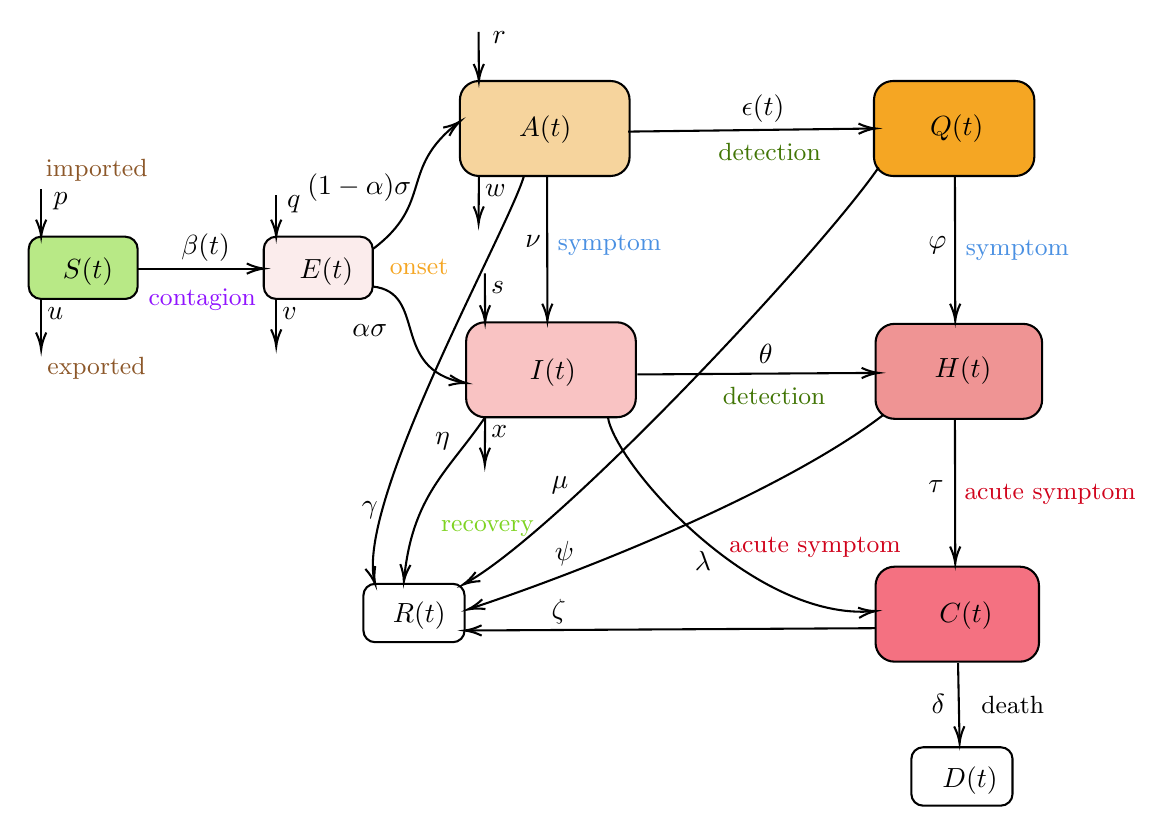
\begin{tikzpicture}[x=0.75pt,y=0.75pt,yscale=-0.75,xscale=0.75]
%uncomment if require: \path (0,592); %set diagram left start at 0, and has height of 592

%Rounded Rect [id:dp09957357672412392] 
\draw  [fill={rgb, 255:red, 184; green, 233; blue, 134 }  ,fill opacity=1 ] (3,196) .. controls (3,191.58) and (6.58,188) .. (11,188) -- (65,188) .. controls (69.42,188) and (73,191.58) .. (73,196) -- (73,220) .. controls (73,224.42) and (69.42,228) .. (65,228) -- (11,228) .. controls (6.58,228) and (3,224.42) .. (3,220) -- cycle ;
%Rounded Rect [id:dp5050898332419083] 
\draw  [fill={rgb, 255:red, 251; green, 236; blue, 236 }  ,fill opacity=1 ] (154,196) .. controls (154,191.58) and (157.58,188) .. (162,188) -- (216,188) .. controls (220.42,188) and (224,191.58) .. (224,196) -- (224,220) .. controls (224,224.42) and (220.42,228) .. (216,228) -- (162,228) .. controls (157.58,228) and (154,224.42) .. (154,220) -- cycle ;
%Straight Lines [id:da4780903246666828] 
\draw    (73,208.5) -- (152,208.5) ;
\draw [shift={(154,208.5)}, rotate = 180] [color={rgb, 255:red, 0; green, 0; blue, 0 }  ][line width=0.75]    (10.93,-3.29) .. controls (6.95,-1.4) and (3.31,-0.3) .. (0,0) .. controls (3.31,0.3) and (6.95,1.4) .. (10.93,3.29)   ;
%Rounded Rect [id:dp054279151026649375] 
\draw  [fill={rgb, 255:red, 246; green, 212; blue, 157 }  ,fill opacity=1 ] (280,100.2) .. controls (280,93.46) and (285.46,88) .. (292.2,88) -- (376.8,88) .. controls (383.54,88) and (389,93.46) .. (389,100.2) -- (389,136.8) .. controls (389,143.54) and (383.54,149) .. (376.8,149) -- (292.2,149) .. controls (285.46,149) and (280,143.54) .. (280,136.8) -- cycle ;
%Rounded Rect [id:dp37056908804655486] 
\draw  [fill={rgb, 255:red, 245; green, 166; blue, 35 }  ,fill opacity=1 ] (546,100.2) .. controls (546,93.46) and (551.46,88) .. (558.2,88) -- (636.8,88) .. controls (643.54,88) and (649,93.46) .. (649,100.2) -- (649,136.8) .. controls (649,143.54) and (643.54,149) .. (636.8,149) -- (558.2,149) .. controls (551.46,149) and (546,143.54) .. (546,136.8) -- cycle ;
%Curve Lines [id:da275515948455739] 
\draw    (224,196) .. controls (263.6,166.3) and (240.47,144.44) .. (278.82,114.9) ;
\draw [shift={(280,114)}, rotate = 503.13] [color={rgb, 255:red, 0; green, 0; blue, 0 }  ][line width=0.75]    (10.93,-3.29) .. controls (6.95,-1.4) and (3.31,-0.3) .. (0,0) .. controls (3.31,0.3) and (6.95,1.4) .. (10.93,3.29)   ;
%Rounded Rect [id:dp899914045285406] 
\draw  [fill={rgb, 255:red, 249; green, 195; blue, 195 }  ,fill opacity=1 ] (284,255.2) .. controls (284,248.46) and (289.46,243) .. (296.2,243) -- (380.8,243) .. controls (387.54,243) and (393,248.46) .. (393,255.2) -- (393,291.8) .. controls (393,298.54) and (387.54,304) .. (380.8,304) -- (296.2,304) .. controls (289.46,304) and (284,298.54) .. (284,291.8) -- cycle ;
%Curve Lines [id:da4853002885061428] 
\draw    (224,220) .. controls (259.64,223.96) and (234.51,273) .. (282.52,281.75) ;
\draw [shift={(284,282)}, rotate = 189.09] [color={rgb, 255:red, 0; green, 0; blue, 0 }  ][line width=0.75]    (10.93,-3.29) .. controls (6.95,-1.4) and (3.31,-0.3) .. (0,0) .. controls (3.31,0.3) and (6.95,1.4) .. (10.93,3.29)   ;
%Straight Lines [id:da9124332231046819] 
\draw    (11,157.5) -- (11,186) ;
\draw [shift={(11,188)}, rotate = 270] [color={rgb, 255:red, 0; green, 0; blue, 0 }  ][line width=0.75]    (10.93,-3.29) .. controls (6.95,-1.4) and (3.31,-0.3) .. (0,0) .. controls (3.31,0.3) and (6.95,1.4) .. (10.93,3.29)   ;
%Straight Lines [id:da12605518772981372] 
\draw    (162,161.5) -- (162,186) ;
\draw [shift={(162,188)}, rotate = 270] [color={rgb, 255:red, 0; green, 0; blue, 0 }  ][line width=0.75]    (10.93,-3.29) .. controls (6.95,-1.4) and (3.31,-0.3) .. (0,0) .. controls (3.31,0.3) and (6.95,1.4) .. (10.93,3.29)   ;
%Straight Lines [id:da03560982385511191] 
\draw    (292,56.5) -- (292.19,86) ;
\draw [shift={(292.2,88)}, rotate = 269.64] [color={rgb, 255:red, 0; green, 0; blue, 0 }  ][line width=0.75]    (10.93,-3.29) .. controls (6.95,-1.4) and (3.31,-0.3) .. (0,0) .. controls (3.31,0.3) and (6.95,1.4) .. (10.93,3.29)   ;
%Straight Lines [id:da550796713766323] 
\draw    (336,149) -- (336.2,240) ;
\draw [shift={(336.2,242)}, rotate = 269.88] [color={rgb, 255:red, 0; green, 0; blue, 0 }  ][line width=0.75]    (10.93,-3.29) .. controls (6.95,-1.4) and (3.31,-0.3) .. (0,0) .. controls (3.31,0.3) and (6.95,1.4) .. (10.93,3.29)   ;
%Straight Lines [id:da12362578932888679] 
\draw    (388,120.5) -- (545,118.53) ;
\draw [shift={(547,118.5)}, rotate = 539.28] [color={rgb, 255:red, 0; green, 0; blue, 0 }  ][line width=0.75]    (10.93,-3.29) .. controls (6.95,-1.4) and (3.31,-0.3) .. (0,0) .. controls (3.31,0.3) and (6.95,1.4) .. (10.93,3.29)   ;
%Rounded Rect [id:dp06713306289293852] 
\draw  [fill={rgb, 255:red, 239; green, 148; blue, 148 }  ,fill opacity=1 ] (547,256.2) .. controls (547,249.46) and (552.46,244) .. (559.2,244) -- (641.8,244) .. controls (648.54,244) and (654,249.46) .. (654,256.2) -- (654,292.8) .. controls (654,299.54) and (648.54,305) .. (641.8,305) -- (559.2,305) .. controls (552.46,305) and (547,299.54) .. (547,292.8) -- cycle ;
%Straight Lines [id:da1253450039391395] 
\draw    (394,276.5) -- (547,275.51) ;
\draw [shift={(549,275.5)}, rotate = 539.63] [color={rgb, 255:red, 0; green, 0; blue, 0 }  ][line width=0.75]    (10.93,-3.29) .. controls (6.95,-1.4) and (3.31,-0.3) .. (0,0) .. controls (3.31,0.3) and (6.95,1.4) .. (10.93,3.29)   ;
%Straight Lines [id:da6862249627192569] 
\draw    (598,149) -- (598.2,240) ;
\draw [shift={(598.2,242)}, rotate = 269.88] [color={rgb, 255:red, 0; green, 0; blue, 0 }  ][line width=0.75]    (10.93,-3.29) .. controls (6.95,-1.4) and (3.31,-0.3) .. (0,0) .. controls (3.31,0.3) and (6.95,1.4) .. (10.93,3.29)   ;
%Rounded Rect [id:dp1447067410775078] 
\draw  [fill={rgb, 255:red, 244; green, 113; blue, 129 }  ,fill opacity=1 ] (547,412.2) .. controls (547,405.46) and (552.46,400) .. (559.2,400) -- (639.8,400) .. controls (646.54,400) and (652,405.46) .. (652,412.2) -- (652,448.8) .. controls (652,455.54) and (646.54,461) .. (639.8,461) -- (559.2,461) .. controls (552.46,461) and (547,455.54) .. (547,448.8) -- cycle ;
%Straight Lines [id:da28419373453425867] 
\draw    (598,305) -- (598.2,396) ;
\draw [shift={(598.2,398)}, rotate = 269.88] [color={rgb, 255:red, 0; green, 0; blue, 0 }  ][line width=0.75]    (10.93,-3.29) .. controls (6.95,-1.4) and (3.31,-0.3) .. (0,0) .. controls (3.31,0.3) and (6.95,1.4) .. (10.93,3.29)   ;
%Curve Lines [id:da3849374732000981] 
\draw    (375,303.5) .. controls (378.98,333.35) and (468.1,435.47) .. (545.83,428.61) ;
\draw [shift={(547,428.5)}, rotate = 534.14] [color={rgb, 255:red, 0; green, 0; blue, 0 }  ][line width=0.75]    (10.93,-3.29) .. controls (6.95,-1.4) and (3.31,-0.3) .. (0,0) .. controls (3.31,0.3) and (6.95,1.4) .. (10.93,3.29)   ;
%Rounded Rect [id:dp8810237408095514] 
\draw   (570,523.5) .. controls (570,519.36) and (573.36,516) .. (577.5,516) -- (627.5,516) .. controls (631.64,516) and (635,519.36) .. (635,523.5) -- (635,546) .. controls (635,550.14) and (631.64,553.5) .. (627.5,553.5) -- (577.5,553.5) .. controls (573.36,553.5) and (570,550.14) .. (570,546) -- cycle ;
%Straight Lines [id:da7788924470393608] 
\draw    (600,462) -- (600.96,511.5) ;
\draw [shift={(601,513.5)}, rotate = 268.89] [color={rgb, 255:red, 0; green, 0; blue, 0 }  ][line width=0.75]    (10.93,-3.29) .. controls (6.95,-1.4) and (3.31,-0.3) .. (0,0) .. controls (3.31,0.3) and (6.95,1.4) .. (10.93,3.29)   ;
%Rounded Rect [id:dp9291512820572525] 
\draw   (218,418.5) .. controls (218,414.36) and (221.36,411) .. (225.5,411) -- (275.5,411) .. controls (279.64,411) and (283,414.36) .. (283,418.5) -- (283,441) .. controls (283,445.14) and (279.64,448.5) .. (275.5,448.5) -- (225.5,448.5) .. controls (221.36,448.5) and (218,445.14) .. (218,441) -- cycle ;
%Curve Lines [id:da7389727414268923] 
\draw    (321,149.5) .. controls (310.11,185.14) and (212.97,357.99) .. (225.1,409.48) ;
\draw [shift={(225.5,411)}, rotate = 253.67000000000002] [color={rgb, 255:red, 0; green, 0; blue, 0 }  ][line width=0.75]    (10.93,-3.29) .. controls (6.95,-1.4) and (3.31,-0.3) .. (0,0) .. controls (3.31,0.3) and (6.95,1.4) .. (10.93,3.29)   ;
%Curve Lines [id:da3764144481947651] 
\draw    (296.2,304) .. controls (272.44,338.65) and (249.46,354.19) .. (244.16,407.86) ;
\draw [shift={(244,409.5)}, rotate = 275.19] [color={rgb, 255:red, 0; green, 0; blue, 0 }  ][line width=0.75]    (10.93,-3.29) .. controls (6.95,-1.4) and (3.31,-0.3) .. (0,0) .. controls (3.31,0.3) and (6.95,1.4) .. (10.93,3.29)   ;
%Curve Lines [id:da8506962083711958] 
\draw    (549,143.5) .. controls (511.19,198.23) and (343.69,377.69) .. (282.91,411.01) ;
\draw [shift={(282,411.5)}, rotate = 331.93] [color={rgb, 255:red, 0; green, 0; blue, 0 }  ][line width=0.75]    (10.93,-3.29) .. controls (6.95,-1.4) and (3.31,-0.3) .. (0,0) .. controls (3.31,0.3) and (6.95,1.4) .. (10.93,3.29)   ;
%Straight Lines [id:da04908465476788049] 
\draw    (547,439.5) -- (285,440.99) ;
\draw [shift={(283,441)}, rotate = 359.66999999999996] [color={rgb, 255:red, 0; green, 0; blue, 0 }  ][line width=0.75]    (10.93,-3.29) .. controls (6.95,-1.4) and (3.31,-0.3) .. (0,0) .. controls (3.31,0.3) and (6.95,1.4) .. (10.93,3.29)   ;
%Curve Lines [id:da10892599229549393] 
\draw    (552,302.5) .. controls (488.32,351.26) and (362.27,401.99) .. (286.14,427.12) ;
\draw [shift={(285,427.5)}, rotate = 341.78999999999996] [color={rgb, 255:red, 0; green, 0; blue, 0 }  ][line width=0.75]    (10.93,-3.29) .. controls (6.95,-1.4) and (3.31,-0.3) .. (0,0) .. controls (3.31,0.3) and (6.95,1.4) .. (10.93,3.29)   ;
%Straight Lines [id:da2069291659666035] 
\draw    (11,228) -- (11,258.5) ;
\draw [shift={(11,260.5)}, rotate = 270] [color={rgb, 255:red, 0; green, 0; blue, 0 }  ][line width=0.75]    (10.93,-3.29) .. controls (6.95,-1.4) and (3.31,-0.3) .. (0,0) .. controls (3.31,0.3) and (6.95,1.4) .. (10.93,3.29)   ;
%Straight Lines [id:da5287473969345702] 
\draw    (162,228) -- (162,256.5) ;
\draw [shift={(162,258.5)}, rotate = 270] [color={rgb, 255:red, 0; green, 0; blue, 0 }  ][line width=0.75]    (10.93,-3.29) .. controls (6.95,-1.4) and (3.31,-0.3) .. (0,0) .. controls (3.31,0.3) and (6.95,1.4) .. (10.93,3.29)   ;
%Straight Lines [id:da7840920125098882] 
\draw    (292.2,149) -- (292.01,177.5) ;
\draw [shift={(292,179.5)}, rotate = 270.38] [color={rgb, 255:red, 0; green, 0; blue, 0 }  ][line width=0.75]    (10.93,-3.29) .. controls (6.95,-1.4) and (3.31,-0.3) .. (0,0) .. controls (3.31,0.3) and (6.95,1.4) .. (10.93,3.29)   ;
%Straight Lines [id:da9543677440180489] 
\draw    (296,211.5) -- (296.19,241) ;
\draw [shift={(296.2,243)}, rotate = 269.64] [color={rgb, 255:red, 0; green, 0; blue, 0 }  ][line width=0.75]    (10.93,-3.29) .. controls (6.95,-1.4) and (3.31,-0.3) .. (0,0) .. controls (3.31,0.3) and (6.95,1.4) .. (10.93,3.29)   ;
%Straight Lines [id:da18449249841812487] 
\draw    (296.2,304) -- (296.01,332.5) ;
\draw [shift={(296,334.5)}, rotate = 270.38] [color={rgb, 255:red, 0; green, 0; blue, 0 }  ][line width=0.75]    (10.93,-3.29) .. controls (6.95,-1.4) and (3.31,-0.3) .. (0,0) .. controls (3.31,0.3) and (6.95,1.4) .. (10.93,3.29)   ;

% Text Node
\draw (23,199.4) node [anchor=north west][inner sep=0.75pt]    {$S( t)$};
% Text Node
\draw (175,199.4) node [anchor=north west][inner sep=0.75pt]    {$E( t)$};
% Text Node
\draw (316,108.4) node [anchor=north west][inner sep=0.75pt]    {$A( t)$};
% Text Node
\draw (580,107.4) node [anchor=north west][inner sep=0.75pt]    {$Q( t)$};
% Text Node
\draw (323,264.4) node [anchor=north west][inner sep=0.75pt]    {$I( t)$};
% Text Node
\draw (180,145.4) node [anchor=north west][inner sep=0.75pt]    {$( 1-\alpha ) \sigma $};
% Text Node
\draw (209,242.4) node [anchor=north west][inner sep=0.75pt]    {$\alpha \sigma $};
% Text Node
\draw (17,157.4) node [anchor=north west][inner sep=0.75pt]    {$p$};
% Text Node
\draw (167,159.4) node [anchor=north west][inner sep=0.75pt]    {$q$};
% Text Node
\draw (299,54.4) node [anchor=north west][inner sep=0.75pt]    {$r$};
% Text Node
\draw (341,185) node [anchor=north west][inner sep=0.75pt]  [font=\small,color={rgb, 255:red, 74; green, 144; blue, 226 }  ,opacity=1 ] [align=left] {symptom};
% Text Node
\draw (99,184.4) node [anchor=north west][inner sep=0.75pt]    {$\beta ( t)$};
% Text Node
\draw (444,126) node [anchor=north west][inner sep=0.75pt]  [font=\small,color={rgb, 255:red, 65; green, 117; blue, 5 }  ,opacity=1 ] [align=left] {detection};
% Text Node
\draw (583,263.4) node [anchor=north west][inner sep=0.75pt]    {$H( t)$};
% Text Node
\draw (447,283) node [anchor=north west][inner sep=0.75pt]  [font=\small,color={rgb, 255:red, 65; green, 117; blue, 5 }  ,opacity=1 ] [align=left] {detection};
% Text Node
\draw (603,188) node [anchor=north west][inner sep=0.75pt]  [font=\small,color={rgb, 255:red, 74; green, 144; blue, 226 }  ,opacity=1 ] [align=left] {symptom};
% Text Node
\draw (586,420.4) node [anchor=north west][inner sep=0.75pt]    {$C( t)$};
% Text Node
\draw (602,345) node [anchor=north west][inner sep=0.75pt]  [font=\small,color={rgb, 255:red, 208; green, 2; blue, 27 }  ,opacity=1 ] [align=left] {acute symptom};
% Text Node
\draw (451,379) node [anchor=north west][inner sep=0.75pt]  [font=\small,color={rgb, 255:red, 208; green, 2; blue, 27 }  ,opacity=1 ] [align=left] {acute symptom};
% Text Node
\draw (233,200.5) node [anchor=north west][inner sep=0.75pt]  [font=\small,color={rgb, 255:red, 245; green, 166; blue, 35 }  ,opacity=1 ] [align=left] {onset};
% Text Node
\draw (320,185) node [anchor=north west][inner sep=0.75pt]    {$\nu $};
% Text Node
\draw (470,254.9) node [anchor=north west][inner sep=0.75pt]    {$\theta $};
% Text Node
\draw (459,94.9) node [anchor=north west][inner sep=0.75pt]    {$\epsilon ( t)$};
% Text Node
\draw (579,185.9) node [anchor=north west][inner sep=0.75pt]    {$\varphi $};
% Text Node
\draw (429,387.9) node [anchor=north west][inner sep=0.75pt]    {$\lambda $};
% Text Node
\draw (579,342.9) node [anchor=north west][inner sep=0.75pt]    {$\tau $};
% Text Node
\draw (588,526.4) node [anchor=north west][inner sep=0.75pt]    {$D( t)$};
% Text Node
\draw (613,481.5) node [anchor=north west][inner sep=0.75pt]  [font=\small,color={rgb, 255:red, 0; green, 0; blue, 0 }  ,opacity=1 ] [align=left] {death};
% Text Node
\draw (581,479.9) node [anchor=north west][inner sep=0.75pt]    {$\delta $};
% Text Node
\draw (235,420.4) node [anchor=north west][inner sep=0.75pt]    {$R( t)$};
% Text Node
\draw (266,368.5) node [anchor=north west][inner sep=0.75pt]  [font=\small,color={rgb, 255:red, 126; green, 211; blue, 33 }  ,opacity=1 ] [align=left] {recovery};
% Text Node
\draw (12,136.5) node [anchor=north west][inner sep=0.75pt]  [font=\small,color={rgb, 255:red, 126; green, 211; blue, 33 }  ,opacity=1 ] [align=left] {\textcolor[rgb]{0.55,0.34,0.16}{imported}};
% Text Node
\draw (78,219.5) node [anchor=north west][inner sep=0.75pt]  [font=\small,color={rgb, 255:red, 144; green, 19; blue, 254 }  ,opacity=1 ] [align=left] {contagion};
% Text Node
\draw (215,355.9) node [anchor=north west][inner sep=0.75pt]    {$\gamma $};
% Text Node
\draw (262,311.9) node [anchor=north west][inner sep=0.75pt]    {$\eta $};
% Text Node
\draw (337,339.9) node [anchor=north west][inner sep=0.75pt]    {$\mu $};
% Text Node
\draw (339,381.9) node [anchor=north west][inner sep=0.75pt]    {$\psi $};
% Text Node
\draw (337,418.9) node [anchor=north west][inner sep=0.75pt]    {$\zeta $};
% Text Node
\draw (13,231.4) node [anchor=north west][inner sep=0.75pt]    {$u$};
% Text Node
\draw (164,231.4) node [anchor=north west][inner sep=0.75pt]    {$v$};
% Text Node
\draw (294.2,152.4) node [anchor=north west][inner sep=0.75pt]    {$w$};
% Text Node
\draw (13,263.5) node [anchor=north west][inner sep=0.75pt]  [font=\small,color={rgb, 255:red, 126; green, 211; blue, 33 }  ,opacity=1 ] [align=left] {\textcolor[rgb]{0.55,0.34,0.16}{exported}};
% Text Node
\draw (298,214.9) node [anchor=north west][inner sep=0.75pt]    {$s$};
% Text Node
\draw (298.2,307.4) node [anchor=north west][inner sep=0.75pt]    {$x$};


\end{tikzpicture}

\caption[Model]{The model consists of following bins: susceptible $S(t)$,, exposed $E(t)$, asymptomatic $A(t)$, symptomatic $I(t)$, quarantined $Q(t)$, isolated $H(t)$,  deceased ($D(t)$ and recovered $R(t)$ individuals in a population of $N(t) = S(t) + E(t) + A(t) + I(t) + Q(t) + H(t) + R(t) + D(t)$ individuals.}
\label{fig1} 
\end{figure*}

The transmission dynamics of COVID-19 in the basic model is given by the following deterministic system of nonlinear differential equations (\ref{eqn:base-model-1})-(\ref{eqn:base-model-10}):
%%
\begin{equation}
\frac{dE}{dt} = q + \beta(t) \left( I + \kappa A + \omega Q + \rho H \right) \frac{S}{N} - \sigma E - v, 
\label{eqn:base-model-1}
\end{equation}
%%
\begin{equation}
\frac{dI}{dt} = s + \alpha \sigma E + \nu A - \left( \eta + \theta + \lambda \right) I - x,
\label{eqn:base-model-2}
\end{equation}
%%
\begin{equation}
\frac{dA}{dt} = r + \left( 1-\alpha \right) \sigma E - \left( \epsilon(t) + \nu + \gamma \right) A - w,
\label{eqn:base-model-3}
\end{equation}
%%
\begin{equation}
\frac{dQ}{dt} = \epsilon(t) A - \left( \varphi + \mu \right) Q,
\label{eqn:base-model-4}
\end{equation}
%%
\begin{equation}
\frac{dH}{dt} = \theta I + \varphi Q - \left( \tau + \psi \right) H ,
\label{eqn:base-model-5}
\end{equation}
%%
\begin{equation}
\frac{dC}{dt} =  \tau H + \lambda I - \left( \delta + \zeta \right) C,
\label{eqn:base-model-6}
\end{equation}
%%
\begin{equation}
\frac{dD}{dt} =  \delta C,
\label{eqn:base-model-7}
\end{equation}
%%
\begin{equation}
\frac{dR}{dt} =  \left( \eta I +  \gamma A + \mu Q + \psi H + \zeta C \right),
\label{eqn:base-model-8}
\end{equation}
%%
\begin{equation}
\frac{dS}{dt} = p -\beta(t) \left( I + \kappa A + \omega Q + \rho H \right) \frac{S}{N} - u,
\label{eqn:base-model-9}
\end{equation}
%%
where,
\begin{equation}
N(t) = S(t) + E(t) + A(t) + I(t) + Q(t) + H(t) + R(t) + D(t),
\label{eqn:base-model-10}
\end{equation}
is the total population. 
\subsubsection{Susceptible individuals: $S(t)$}
In our model, the susceptible individuals gets exposed to infection, and move to exposed group $E(t)$, from coming in contact with an infected individual, who may be symptomatic, asymptomatic, quarantined, or isolated. $\beta(t)$ is the baseline infectious contact rate, which can vary with time or assumed constant for the analysis of our baseline model. We assume that a person who is infected with symptom, and is not isolated, has the basic transmission coefficient of $\beta(t)$, that is changing over time. Based on \cite{TANG2020248, EIKENBERRY2020293}, we define $\beta(t)$ to have a value $\beta_0$ till time $t_0$ and then as a decreasing function with respect to time $t$, to reaching $\beta_{\min}$. 
\begin{equation}
\beta(t) = 
\begin{cases}
\beta_0 & t < t_0 \\
\beta_{\min} + \left( \beta_0 - \beta_{\min}\right) e^{-r\left( t - t_0\right) } & t \geq t_0
\end{cases}
\label{eqn:base-model-11}
\end{equation}
We would like to note that in certain countries, stringency measures were in place at an earlier stages of the epidemic and was relaxed over time leading to a higher contact rate. Under such scenario, we use value $\beta_0$. 

Our model incorporates some facets of mobility, whereby, we recruit a inflow of susceptible individuals into the region at a rate $p$, and also consider an outflow with a rate $u$. It is well known that such inflow of travelers in the community including regional migration, immigration and emigration has lead to faster spread of the contagion [Citation]. A similar inflow and outflow has been amended to exposed, symptomatic and  asymptomatic but undetected compartments, namely $E(t), A(t), I(t)$. In the absence of an effective screening test, and when it was observed that in the wake of governmental stringency measure, people tried to flee regions that are under stricter measures, individuals from these  groups carried contagion to other geographic regions [citation]. 

We assume that the asymptomatic individuals infect with a lower contact rate ($\kappa < 1$) than the symptomatic individuals. Once someone symptomatic is diagnosed, they can only infect healthcare workers and this lower contact rate is captured by the parameter ($\rho < 1$). Similarly, quarantined individuals have much lower contact rate of ($\omega < 1$). Overall rate of change for the susceptible population is thus defined by equation (\ref{eqn:base-model-9}).

\subsubsection{Exposed individuals: $E(t)$}
Individuals in compartment $E$, are exposed to the virus, and are not contagious during a period of latent time. An individual in $E$ becomes infectious, and moves to compartment $A$ as asymptomatic or to $I$ as symptomatic. We assume that $\sigma$ is the transition rate from exposed to infectious, and a fraction $\alpha$ of them show symptoms. Overall rate of change for the exposed population is thus defined by equation (\ref{eqn:base-model-1}).

\subsubsection{Symptomatic individuals: $I(t)$}
Symptomatic individuals can get diagnosed ($\theta$) and be isolated, or show acute symptoms and be hospitalized ($\lambda$), or can recover at the rate $\eta$. It has been observed that $\eta \geq \gamma$, where symptomatic individuals recover at faster rate than asymptomatic individuals, and asymptomatic individuals have longer duration of viral shedding \cite{Long2020}. Overall rate of change is given by equation (\ref{eqn:base-model-2}).

\subsubsection{Asymptomatic individuals: $A(t)$}
Asymptomatic individuals can enter into population with rate $r$, and then can migrate out at rate $w$. Asymptomatic individuals can eventually show symptoms and move to $I$ at rate $\nu$ or can have a positive diagnosis and move to quarantine. We model testing of asymptomatic population as a function of time as the community testing process ramps up. Testing rate has been captured as $\epsilon(t)$. Finally, they can recover at the rate $\gamma$. Overall rate of change is given by equation (\ref{eqn:base-model-3}).

\subsubsection{Quarantined individuals: $Q(t)$}
Quarantined individuals are asymptomatic population after diagnosis and they have very low contact rate ($\omega < 1$). This is mostly by infecting the other family members or by breach of protocol. They however, may develop symptoms and move to $H$ or recover. Overall rate of change is given by equation (\ref{eqn:base-model-4}).

\subsubsection{Isolated individuals: $H(t)$}
Isolated individuals are showing symptoms and has been either home isolated or has been hospitalized. They can pass the infection to a limited number of health care professional or caregiver ($\rho$). They can become critical and require treatments in intensive care ($\tau$), and a large number of them recover ($\psi$). Overall rate of change is given by equation (\ref{eqn:base-model-5}).

\subsubsection{Critical, Recovered and Deceased individuals: $C(t), R(t), D(t)$}
These counters collect information on population that are critical, recovered or have deceased. Overall rate of change is given by equations (\ref{eqn:base-model-6}) -  (\ref{eqn:base-model-8}). We assume that recovered individuals possess lasting immunity against SARS-CoV-2 over the period of simulation.

\subsubsection{Baseline epidemiological parameters}
In this section we describe the estimated values of various parameters based on the current literature. It has been noted in the literature that the clinical course of the disease is typically quite long. Average total duration of illness has been estimated to be three weeks in \cite{Zhou2020}. In the baseline model we consider $p, q, r, s, u, v, w, x$ to be 0. In other words we do  not include any mobility in the base model. In following we will include them in the extended model with appropriate meaning. Parameter $\beta_0$ is strongly dependent on the population behavior. We select a default value that has been estimated in \cite{Shen2020.01.23.916726} for pre-lockdown period.

\cite{Long2020}


	\begin{table*}
	\centering
	\begin{tabularx}{\textwidth}[t]{p{0.09\textwidth}p{0.35\textwidth}p{0.3\textwidth}p{0.15\textwidth}}
		\hline
		\textbf{Param} &  \textbf{Description} &  \textbf{Possible Range} &  \textbf{Default}\\ [0.5ex]
		\hline
		$\beta_0$ &  infectious contact rate & $0.5$-$1.5$ $ day^{-1}$ \cite{Li489,Shen2020.01.23.916726} & $0.76$ $day^{-1}$\\
		\hline
		$\kappa$ &  infectiousness factor asymptomatic & $0.4$-$0.6$ \cite{Li489,Ferguson2020} & $0.5$\\
		\hline
		$\omega$ &  infectiousness factor quarantined & $0.005$-$0.011$ \cite{Giordano2020} & $0.011$\\
		\hline
		$\rho$ &  infectiousness factor isolated & $0.005$-$0.011$ \cite{Giordano2020} & $0.011$\\
		\hline
		$\sigma$ &  transition rate exposed to infectious & $1/14$-$1/3$ $day^{-1}$ \cite{Li489,Lauer2020.02.02.20020016} & $1/5.2$ $day^{-1}$\\
		\hline
		$\alpha$ &  fraction of infections that become symptomatic & $0.15$-$0.7$  \cite{Li489,Ferguson2020,Moriarty2020} & $0.5$\\
		\hline
		$\nu$ &  transition rate  asymptomatic to symptomatic & $0.025$-$0.125$ \cite{Giordano2020} & $0.125$\\
		\hline
		$\epsilon_0$ &  detection rate asymptomatic & $0.171$ \cite{Giordano2020} & $0.171$ \\
		\hline
		$\varphi$ &  rate of asymptomatic developing symptoms & $0.025$-$0.125$ \cite{Giordano2020} & $0.125$\\
		\hline
		$\theta$ &  rate of detection of symptomatic & $0.371$ & $0.371$\\
		\hline
		$\tau$ &  rate of developing life-threatening symptoms in isolation & $0.027$ & $0.027$\\
		\hline
		$\lambda$ &  rate of developing life-threatening symptoms for symptomatic& $0.017$ & $0.017$\\
		\hline
		$\gamma$ &  recovery rate of asymptomatic & $0.034$ & $0.034$\\
		\hline
		$\eta$ &  recovery rate of symptomatic & $0.017$ & $0.017$\\
		\hline
		$\mu$ &  recovery rate of quarantined & $0.034$ & $0.034$\\
		\hline
		$\psi$ & recovery rate of isolated & $0.017$ & $0.017$\\
		\hline
		$\zeta$ &  recovery rate of critical & $0.017$ & $0.017$\\
		\hline
		$\delta$ &  mortality rate & $0.01$-$0.015$ & $0.015$\\ [1ex] 
		\hline
	\end{tabularx}
	\caption{Baseline parameters, brief description, possible ranges based on modeling and clinical studies, and default value chosen for this study.}
	\label{Table1}
\end{table*}

\subsubsection{The basic reproduction number for baseline model}
The basic reproduction number is calculated for the special case when we have $\beta(t) = \beta_0, \epsilon(t) = \epsilon_0$, and $p = q = r = s = u = v = w = x = 0$. in following we explore the local stability of the disease-free equilibrium (DFE) using the next generation operator method \cite{Diekmann1990,VANDENDRIESSCHE200229}. Following \cite{VANDENDRIESSCHE200229}, we define the system of equations (\ref{eqn:base-model-1})-(\ref{eqn:base-model-10}), in more compact form as:
%
%
\begin{equation}
\dot{X} = f(X) = \mathcal{F}(X) - \mathcal{V}(X), 
\label{eqn:baseline-compact-1}
\end{equation}
%
%
where, $X = \left( E, I, A, Q, H, C, D, R, S \right)^t $, and $\mathcal{F}(X) $ containing rate of appearance of new infections defined as:
%
%
\begin{equation}
\mathcal{F}(X) = 
\begin{pmatrix}
\beta_0 \left( I + \kappa A + \omega Q + \rho H \right) \frac{S}{N} \\
0\\
0\\
0\\
0\\
0\\
0\\
0\\
0
\end{pmatrix}, 
\label{eqn:baseline-compact-2}
\end{equation}
%
%
and, $\mathcal{V}(X)$ capturing the movement between the compartments, with $\mathcal{V}^{-}(X)$ as the rate of outward transfer, and $\mathcal{V}^{+}(X)$ as the rate of inward transfer for each compartment, we have,
%
%
\begin{equation}
\begin{split}
\mathcal{V}(X) &= \mathcal{V}^{-}(X) - \mathcal{V}^{+}(X)\\
&= \begin{pmatrix}
\sigma E \\
\left( \eta + \theta + \lambda \right) I\\
\left( \epsilon_0 + \nu + \gamma \right) A\\
\left( \varphi + \mu \right) Q\\
\left( \tau + \psi \right) H\\
\left( \delta + \zeta \right) C\\
0\\
0\\
\beta_0 \left( I + \kappa A + \omega Q + \rho H \right) \frac{S}{N}
\end{pmatrix} - 
\begin{pmatrix}
0 \\
\alpha \sigma E + \nu A\\
\left( 1 - \alpha \right)\sigma E  \\
\epsilon_0 A\\
\theta I + \varphi Q\\
\tau H + \lambda I\\
\delta C\\
\left( \eta I +  \gamma A + \mu Q + \psi H + \zeta C \right)\\
0
\end{pmatrix}\\
&= \begin{pmatrix}
\sigma E \\
\left( \eta + \theta + \lambda \right) I - \alpha \sigma E - \nu A\\
\left( \epsilon_0 + \nu + \gamma \right) A - \left( 1 - \alpha \right)\sigma E\\
\left( \varphi + \mu \right) Q - \epsilon_0 A\\
\left( \tau + \psi \right) H - \theta I - \varphi Q\\
\left( \delta + \zeta \right) C - \tau H - \lambda I\\
-\delta C\\
-\left( \eta I +  \gamma A + \mu Q + \psi H + \zeta C \right)\\
\beta_0 \left( I + \kappa A + \omega Q + \rho H \right) \frac{S}{N}
\end{pmatrix}
\end{split}
\label{eqn:baseline-compact-3}
\end{equation}
%
%
We also define $\mathcal{X}_s$, as the set of all possible disease free states. In order to directly apply the results in \cite{VANDENDRIESSCHE200229}, following shall hold for equation $\dot{X} = f(x) = \mathcal{F}(X) - \mathcal{V}(X)$:
\begin{enumerate}
	\item Functions $\mathcal{F}(X)$, $\mathcal{V}^{-}(X)$ and $\mathcal{V}^{+}(X)$, are all non-negative, when $X > 0$.
	\item If $X \in \mathcal{X}_s$, then $\mathcal{V}^{-}(x)=\mathcal{F}(x)=\mathcal{V}^{+}(x)=0$ for $x \in \{E, I, A, Q, H, C, D, R\}$.
	\item Let $Df(X_0)$ be the Jacobian matrix evaluated at DFE $X_0$, and defined as the partial derivative $[{\partial f}/{\partial x}]$ for $x \in \{E, I, A, Q, H, C, D, R, S\}$. If $\mathcal{F}(X) = 0$, then all eigenvalues of $Df(X_0)$ has negative real parts.
\end{enumerate}
We note that each function represents a directed transfer of individuals, and they are all non-negative. (1) and (2), can be observed from the equations (\ref{eqn:baseline-compact-2}) and (\ref{eqn:baseline-compact-3}).  For (3), setting $\mathcal{F}(X) = 0$, we consider linearized system $\dot{X} = - D\mathcal{V}(X_0)(X-X_0)$, near DFE. From equation (\ref{eqn:DFE-3}) we observe that eigenvalues corresponding to $Df(X_0)$ has zero eigenvalues of multiplicity $3$ with associated eigenvectors in the directions of $D, R, S$. The results in \cite{VANDENDRIESSCHE200229} still holds for our system for stability in the directions of the susceptible and recovered compartment (note that )as $D$ is a counting compartment), this however, has no consequence in the meaning of the threshold $\mathcal{R}_0$. In fact this technicality can be resolved by adding natural birth and death rates proportional to the compartments $S$ and $R$ that is arbitrarily small and positive. 
%
%
Let $X_0 \in \mathcal{X}_s$ be a DFE. Then $X_0 = \left( 0, 0, 0, 0, 0, 0, 0, 0, S_0 \right) $, and with $S_0/N_0=1$ we have, 
%
%
\begin{equation}
\begin{split}
D \mathcal{F}(X_0) \\
&=  \begin{pmatrix}
0 & \beta_0 & \kappa \beta_0 & \omega \beta_0 & \rho \beta_0 & 0 & 0 & 0 & 0 \\
0 & 0 & 0 & 0 & 0 & 0 &0 & 0 &0 \\
0 & 0 & 0 & 0 & 0 & 0 &0 & 0 &0 \\
0 & 0 & 0 & 0 & 0 & 0 &0 & 0 &0 \\
0 & 0 & 0 & 0 & 0 & 0 &0 & 0 &0 \\
0 & 0 & 0 & 0 & 0 & 0 &0 & 0 &0 \\
0 & 0 & 0 & 0 & 0 & 0 &0 & 0 &0 \\
0 & 0 & 0 & 0 & 0 & 0 &0 & 0 &0 \\
0 & 0 & 0 & 0 & 0 & 0 &0 & 0 &0
 \end{pmatrix}\\
 &=  \begin{pmatrix}
 F & 0\\
 0 & 0
  \end{pmatrix}
\end{split}
\label{eqn:DFE-1}
\end{equation}
%
%
With,
%
%
\begin{equation}
F = \begin{pmatrix}
0 & \beta_0 & \kappa \beta_0 & \omega \beta_0 & \rho \beta_0 \\
0 & 0 & 0 & 0 & 0\\
0 & 0 & 0 & 0 & 0\\
0 & 0 & 0 & 0 & 0\\
0 & 0 & 0 & 0 & 0
  \end{pmatrix}
  \label{eqn:DFE-2}
\end{equation}
%
%
Similarly, we have 
%
%
\begin{equation}
\begin{split}
D \mathcal{V}(X_0) = \\
\begin{pmatrix}
\sigma & 0 & 0 & 0 & 0 & 0 &0 & 0 &0 \\
-\alpha \sigma & \left( \eta + \theta + \lambda\right)  & - \nu & 0 & 0 & 0 &0 & 0 &0 \\
-\left( 1- \alpha \right) \sigma & 0 & \left( \epsilon_0 + \nu + \gamma \right) & 0 & 0 & 0 &0 & 0 &0 \\
0 & 0 & - \epsilon_0 & \left( \varphi + \mu\right)  & 0 & 0 &0 & 0 &0 \\
0 & -\theta & 0 & -\varphi & \left( \tau + \psi\right)  & 0 &0 & 0 &0 \\
0 & -\lambda & 0 & 0 & -\tau & \left( \delta + \zeta\right)  &0 & 0 &0 \\
0 & 0 & 0 & 0 & 0 & -\delta &0 & 0 &0 \\
0 & -\eta & -\gamma & -\mu & -\psi & -\zeta &0 & 0 &0 \\
0 & \beta_0 & \kappa\beta_0 & \omega\beta_0 & \rho\beta_0 & 0 &0 & 0 &0
  \end{pmatrix}\\
  =\begin{pmatrix}
  V & 0\\
  J_3 & J_4
  \end{pmatrix}
\end{split}
\label{eqn:DFE-3}
\end{equation}
%
%
With,
%
%
\begin{equation}
V = \begin{pmatrix}
\sigma & 0 & 0 & 0 & 0 \\
-\alpha \sigma & \left( \eta + \theta + \lambda\right)  & - \nu & 0 & 0 \\
-\left( 1- \alpha \right) \sigma & 0 & \left( \epsilon_0 + \nu + \gamma \right) & 0 & 0 \\
0 & 0 & - \epsilon_0 & \left( \varphi + \mu\right)  & 0 \\
0 & -\theta & 0 & -\varphi & \left( \tau + \psi\right)
\end{pmatrix}
\label{eqn:DFE-4}
\end{equation}
%
%
Defining $\rho(A) = \max {\{ | \lambda_1 |, \ldots,  | \lambda_n |\} }$ as the spectral radius of an $n \times n$ matrix $A$, with eigenvalues $\lambda_1 \ldots \lambda_n$, and $|\dot|$ denoting absolute values. According to \cite{VANDENDRIESSCHE200229}, basic reproduction number $\mathcal{R}_0$ associated to the system can be computed as $\mathcal{R}_0 = \rho(FV^{-1})$. Hence, based on the discussion above, for the baseline model we have,
%
%
\begin{equation}
\mathcal{R}_0 = 
\label{eqn:Rnot}
\end{equation}
%
%
\subsection{Extending the baseline model}
In this section we consider various extension of the model and parameters. First extension is to model confinement - where a large proportion of susceptible population is placed under restricted movement, and thereby reducing the probability of contact. Such restriction has been modeled by introducing another compartment $L$. Individuals from $S$ move to $L$ at rate $u(t)$. In many countries, confinement was spread over several weeks followed by a period of de-confinement. We model de-confinement by individuals moving from $L$ to $S$ at rate $p(t)$. In specific we modify equation (\ref{eqn:base-model-9}) as follows
%%
\begin{equation}
\frac{dS}{dt} = p(t)L -\beta(t) \left( I + \kappa A + \omega Q + \rho H \right) \frac{S}{N} - u(t)S,
\label{eqn:lockdown-model-1}
\end{equation}
%
%
We also add following dynamics to the baseline model 
%%
\begin{equation}
\frac{dL}{dt} = u(t)S - p(t)L,
\label{eqn:lockdown-model-2}
\end{equation}
%%
Thus, equations (\ref{eqn:base-model-1}-\ref{eqn:base-model-8}), equation (\ref{eqn:lockdown-model-1}), and (\ref{eqn:lockdown-model-2}) along with equation (\ref{eqn:base-model-10}), defines the confinement - de-confinement scenario. A few remarks are in place for the time dependent functions $u(t)$ and $p(t)$.

\section*{Authors' contributions}
\label{SEC5}

%% References
\bibliographystyle{elsarticle-num}
\bibliography{covid_m.bib}	
\end{document}

%%
%% End of file `elsarticle-template-2-harv.tex'.
